\pdfoutput=1
\pdfinfoomitdate=1
\pdftrailerid{}
\pdfsuppressptexinfo=15
\documentclass[11pt]{article}
\makeatletter
\def\input@path{{vendor/}}
\makeatother
\usepackage[utf8]{inputenc}
\usepackage[margin=1in]{geometry}
\usepackage{amsmath,amssymb,amsthm,mathtools}
\usepackage{booktabs,enumitem,microtype}
\usepackage{xcolor}
\usepackage{tikz}
\usetikzlibrary{arrows.meta,positioning}
\usepackage[colorlinks=true,linkcolor=blue!45!black,citecolor=blue!45!black,urlcolor=blue!45!black]{hyperref}
\usepackage[nameinlink,noabbrev]{cleveref}
\usepackage{bookmark}
\crefname{theorem}{Theorem}{Theorems}
\crefname{lemma}{Lemma}{Lemmas}
\crefname{proposition}{Proposition}{Propositions}
\crefname{corollary}{Corollary}{Corollaries}
\crefname{section}{Section}{Sections}
\crefname{equation}{Equation}{Equations}
\crefname{figure}{Figure}{Figures}
\hypersetup{pdftitle={The Factor-Two Hardness Threshold for Vertex Cover},pdfauthor={OpenAI},pdfsubject={A deterministic gap reduction from Label Cover}}
\numberwithin{equation}{section}
\newtheorem{theorem}{Theorem}[section]
\newtheorem{lemma}[theorem]{Lemma}
\newtheorem{proposition}[theorem]{Proposition}
\newtheorem{corollary}[theorem]{Corollary}
\theoremstyle{definition}
\newtheorem{definition}[theorem]{Definition}
\theoremstyle{remark}
\newtheorem{remark}[theorem]{Remark}
\newcommand{\E}{\mathbb E}
\DeclareMathOperator{\Var}{Var}
\DeclareMathOperator{\Ent}{H}
\DeclareMathOperator{\KL}{D}
\DeclareMathOperator{\TV}{TV}
\DeclareMathOperator{\val}{val}
\DeclareMathOperator{\supp}{supp}
\DeclareMathOperator{\conv}{conv}
\DeclareMathOperator{\dist}{dist}
\newcommand{\norm}[1]{\left\|#1\right\|_*}
\newcommand{\abs}[1]{\left|#1\right|}
\newcommand{\ceil}[1]{\left\lceil#1\right\rceil}
\newcommand{\floor}[1]{\left\lfloor#1\right\rfloor}
\newcommand{\ind}{\mathbf 1}
\newcommand{\R}{\mathbb R}
\newcommand{\Ftwo}{\mathbb F_2}
\setlist[enumerate]{itemsep=3pt,topsep=5pt}
\setlist[itemize]{itemsep=3pt,topsep=5pt}
\emergencystretch=1.2em
\clubpenalty=10000
\widowpenalty=10000
\displaywidowpenalty=10000

\title{The Factor-Two Hardness Threshold for Vertex Cover}
\author{OpenAI}
\date{September 23, 2026}

\begin{document}
\maketitle
\begin{abstract}
We prove that minimum Vertex Cover is NP-hard to approximate within
every fixed factor below two, even on simple unweighted graphs.
\end{abstract}

\section{Introduction}
\label{sec:introduction}

A vertex cover of a graph is a set of vertices meeting every edge.
Its complement is an independent set, a set containing no two adjacent
vertices. This elementary duality lets us express the hardness gap
in terms of the densities of independent sets.
For a finite simple undirected graph \(G\), write \(\tau(G)\) for
the minimum size of a vertex cover and \(n=|V(G)|\). An
\(\alpha\)-approximation returns an actual cover of size at most
\(\alpha\tau(G)\). The endpoints of a maximal matching give a
factor-\(2\) approximation. We prove that every fixed improvement
in this factor is NP-hard.

\begin{theorem}[Explicit cover gap]
\label{thm:gap}
For every fixed integer \(m\geq4\), there is a deterministic
polynomial-time reduction from \(\mathrm{3SAT}\) to finite simple
undirected unweighted graphs with the following guarantees:
\[
\begin{array}{ll}
\text{the formula is satisfiable}
 &\Longrightarrow\quad
 \tau(G)<\left(\dfrac12+\dfrac1m\right)|V(G)|,\\[6pt]
\text{the formula is unsatisfiable}
 &\Longrightarrow\quad
 \tau(G)>\left(1-\dfrac1m\right)|V(G)|.
\end{array}
\]
The output lists all vertices and edges explicitly.
\end{theorem}

\begin{corollary}
\label{thm:hardness}
For every fixed real \(\alpha\) with \(1\leq\alpha<2\),
approximating Vertex Cover within factor \(\alpha\) is NP-hard.
Thus, unless \(\mathrm P=\mathrm{NP}\), no deterministic
polynomial-time algorithm achieves factor \(2-\varepsilon\)
for any fixed \(\varepsilon\in(0,1]\).
\end{corollary}

The ratio of the two thresholds is \(2-6/(m+2)\), which tends to
\(2\). The reduction is polynomial for each fixed \(m\); its
constants are allowed to depend on the desired approximation factor.
We prove the approximation consequence, including an exact rational
separating threshold, in \Cref{sec:conclusion}.

\subsection{Historical context and the role of the method}

Vertex Cover appeared as \textsc{Node Cover} among the problems
Karp proved NP-complete in 1972~\cite{Karp1972}. Exact hardness
still leaves room for approximation, and the elementary
maximal-matching algorithm achieves factor two. Subsequent algorithms
improved this ratio by an amount depending on the graph order.
Karakostas obtained \(2-\Theta(1/\sqrt{\log n})\) using semidefinite
programming~\cite{Karakostas2009}. This saving tends to zero as
\(n\) grows. The threshold addressed here concerns a fixed saving
below two, so it is compatible with such algorithmic improvements.

The connection between proof checking and approximation hardness
was developed by Feige, Goldwasser, Lov\'asz, Safra, and
Szegedy~\cite{FGLSS96}. Their graph encodes accepting local proof
views, with consistency of the answers governing adjacency.
The PCP breakthrough of 1992, developed by Arora and Safra and
completed in constant-query form by Arora, Lund, Motwani, Sudan,
and Szegedy~\cite{AroraSafra98,ALMSS98}, yielded constant
approximation gaps for problems including Vertex Cover. Raz's
parallel repetition theorem~\cite{Raz1998} reduces the soundness
of projection games to any desired fixed positive constant while
preserving perfect completeness. Together these results supply the
Label Cover promise stated precisely in \Cref{src:hardness}, the
only external hardness input used here.

For Vertex Cover, H{\aa}stad established hardness for every fixed
factor below \(7/6\)~\cite[Theorem~8.1]{Hastad2001}.
Dinur and Safra raised this to every fixed factor below
\(10\sqrt5-21\), approximately \(1.36068\)~\cite[Theorem~1.1]{DinurSafra2005}.
Their analysis uses biased set families and Boolean-function
structure to control independent-set density. Khot's Unique Games
Conjecture~\cite{Khot02} proposed a stronger source of approximation
gaps. Assuming this conjecture, Khot and Regev obtained hardness
for every fixed factor below two~\cite{KhotRegev2008}. Their proof
uses a biased long code and an equivalent, stronger formulation
of the source promise that supports short lists of candidate labels.
Friedgut's approximation theorem for Boolean functions of low
average sensitivity~\cite{Friedgut1998} supplies bounded sets of
relevant coordinates in that analysis.

The 2017--2018 developments in the \(2\)-to-\(2\) Games program
gave an unconditional advance. The Grassmann-graph reduction of Khot, Minzer, and
Safra~\cite{KhotMinzerSafra2025}, the work of Dinur, Khot, Kindler,
Minzer, and Safra~\cite{DKKMS2025}, and the contribution of Barak,
Kothari, and Steurer~\cite{BarakKothariSteurer2019} culminated in
the expansion theorem of Khot, Minzer, and
Safra~\cite{KhotMinzerSafra2023}. This completed the Games Theorem
with imperfect completeness and yielded unconditional Vertex Cover
hardness for every fixed factor below \(\sqrt2\). The resulting
independent-set gap has completeness density close to
\(1-1/\sqrt2\) and arbitrarily small soundness density. The gap
in \Cref{thm:gap} instead has completeness density approaching
\(1/2\), which is what gives the factor-two threshold.

Our argument retains the objective of extracting short local label
lists from a large independent set, but obtains the lists from
Lipschitz derivatives. The central step preserves variance while
restricting the information available to each list. We adapt the
product-space orthogonal decomposition of the Efron--Stein
method~\cite[Section~2]{EfronStein1981}, combining it with a
resampling estimate that controls the loss caused by this information
restriction. A variance inequality on a product of intervals then
supplies gradient energy, from which short candidate-label lists can
be extracted without an alphabet-size factor. These ingredients
are proved in full in \Cref{sec:restriction,ana:private-section};
the final decoding uses the ordinary Label Cover promise above.


\subsection{The construction and the soundness mechanism}

A Label Cover instance is a bipartite constraint system: every edge
asks that a specified map send the label on its left endpoint to the
label on its right endpoint. Its value is the largest fraction of
constraints satisfied by one assignment of labels to all variables.
Our source promise separates value one from arbitrarily small fixed
value. The alphabets may grow as that fixed value decreases; our
analytic estimates will not depend on their sizes.
The exact source theorem is stated in \Cref{src:hardness}.

Imagine \(d\) positions, with an independent source constraint
assigned to each unordered pair. At a pair \(j<k\), position
\(j\) receives the constraint's left endpoint and position \(k\)
its right endpoint. A position's \emph{query} is its type together
with these \(d-1\) endpoint questions. It does not reveal constraint
indices or opposite endpoints. A local label assigns symbols to the
variables in one query and satisfies every source constraint internal
to that scope. A compatible family chooses at most one label per query;
its members agree on overlaps and satisfy every constraint internal
to their combined scopes.

Give one vector coordinate to each query--label pair. A compatible
family acts on a vector by summing the coordinates it selects; the
largest absolute value of these sums defines a norm,
\(\norm{\cdot}\). At each position, a vector of grid weights is
supported on that position's query block. A graph vertex specifies
all pair constraints and all position weights. Let \(S_v\) be
the sum of its position vectors. For a positive threshold \(t\),
distinct vertices \(v,w\) are adjacent precisely when
\(\norm{S_v+S_w}\leq2t\).

A satisfying source assignment restricts to compatible labels for
every query. Its linear functional exceeds \(t\) on an independent
set: on the sum of two such vertices it exceeds \(2t\). A tail
estimate for a sum of symmetric weights shows that this set occupies
nearly half the graph. \Cref{graph:section} gives the construction,
its deterministic implementation, and this completeness argument.

\paragraph{Why endpoint information matters.}
For soundness, we will extract short lists of local labels from a
large independent set. Each list must depend only on its position's
own query and weights. To see why, fix a pair of positions and all
data except their shared source constraint. Each of the two lists
then varies only with its own endpoint of that constraint. Choosing
one rank in each list defines a labeling of all source variables,
so source soundness bounds the probability that these two labels are
compatible. This argument fails if either list also sees the opposite
endpoint or the occurrence index. The main task is therefore to
obtain both enough compatibility among the lists and this restriction
on their information.

\paragraph{Retaining variance in own-question means.}
Discard from a large independent set its at most one vertex with
vector norm at most \(t\). The remaining vectors are separated
from the negatives of one another. The half-difference of their
distance functions gives one fixed odd Lipschitz function \(F\).
Replace the grid weights by independent continuous uniform weights
on cubes; rounding and the Lipschitz bound control the error.
On fresh random sums, \(F\) then has variance at least a fixed
multiple of \(d\), as proved in \Cref{ana:function}.

Choose a small batch \(J\) of \(h\) positions, freeze the
weights outside it and the constraints on pairs not contained in it,
and average \(F\) conditional only on one remaining position's
own endpoint questions and weights. Such averaging might erase the
variance. \Cref{res:private-variance} shows that a suitable
restriction retains total variance at least a fixed multiple of
\(h\) in these own-question means. The proof decomposes over the independent weights
and pair seeds. Its crucial estimate resamples every seed incident
to one position while preserving the questions received at all other
positions. Only the first position's query can then change. This
bounds the energy lost when the conditional means forget other
positions' questions, independently of the label alphabets.

\paragraph{From variance to compatible lists.}
For fixed batch queries, differentiate \(F\) composed with the
sum of the position vectors. The full gradient lies in the convex
hull of signed incidence vectors of compatible label selections
(\Cref{ana:gradient}). It carries a compatible representation, but
can depend on all batch inputs. Conversely, the derivatives of the
own-question means have the required information restriction, but
need not together lie in that same hull.

The cube variance bound in \Cref{ana:cube} gives enough squared
energy in the own-question gradients. Each block has \(\ell^1\)
norm at most one, so thresholding its entries produces a short list
without an alphabet-size factor. Conditional Jensen then transfers
the retained list mass back to the single full gradient before its
compatible-incidence bound is used. If \(Z\) is the largest
number of lists hit by one compatible selection, this gives
\(\E Z\geq2\) (\Cref{ana:lists}). The pair-decoding argument
above, summed over pairs of positions, gives \(\E Z<3/2\)
under source soundness (\Cref{dec:pair}), a contradiction.

\paragraph{Organization.}
\Cref{sec:source} states the source promise and introduces the
construction parameters.
\Cref{graph:section} constructs the graph and proves completeness;
\Cref{ana:section} converts an independent set into the analytic
input. The restriction, gradient, and decoding arguments occupy
\Cref{sec:restriction,ana:private-section,dec:section}, respectively.
\Cref{sec:conclusion} verifies a joint choice of all parameters and
turns the density gap into the approximation threshold.

The construction enumerates all its finite seeds and grid weights.
Random variables describe the uniform distribution on this output
and appear only in its analysis. Neither the independent set, the
function \(F\), nor the conditional means need to be computed by
the reduction.


\section{The source problem and construction parameters}
\label{sec:source}

Write \([k]=\{1,\ldots,k\}\). A \emph{Label Cover instance}
\(\Phi\) consists of two disjoint finite variable sets \(U,V\),
two nonempty finite alphabets \(\Sigma_U,\Sigma_V\), and an explicit
nonempty list of \(M\) constraint occurrences. Occurrence \(c\in[M]\)
has endpoints \(x_c\in U\), \(y_c\in V\), and a total map
\(\pi_c:\Sigma_U\to\Sigma_V\). A labeling \(A\) assigns each
variable a symbol from its side's alphabet. It satisfies occurrence
\(c\) when
\[
  \pi_c(A(x_c))=A(y_c).
\]
The value \(\val(\Phi)\) is the maximum fraction of satisfied
occurrences. List entries count with their multiplicity. Endpoints
and map tables are given explicitly in binary; unused variable
declarations can be removed. We require no regularity or expansion
condition on the constraint graph.

\begin{theorem}[Perfect-completeness Label Cover hardness]
\label{src:hardness}
For every fixed rational \(\sigma\in(0,1)\), there are nonempty
constant alphabets and a deterministic polynomial-time reduction
from \(\mathrm{3SAT}\) to instances of the form above such that
satisfiable formulas give \(\val(\Phi)=1\), and unsatisfiable
formulas give \(\val(\Phi)\leq\sigma\).
\end{theorem}

This is the standard consequence of the probabilistically checkable
proof (PCP) theorem~\cite{AroraSafra98,ALMSS98} and parallel
repetition~\cite{Raz1998}.
A quantitative formulation appears in the full version of Dinur
and Steurer~\cite[Theorem~6.2]{DinurSteurer2014}.
The precise unweighted, total-projection formulation is
recorded in \cite[Definitions~1.1--1.2 and Theorem~1.3]{DKKMS2025}.
There the constraints are even \(D\)-to-one for a suitable constant
\(D\), a property we do not use. The constants, including the
alphabets and \(D\), may depend on \(\sigma\). This theorem is the
only external hardness input to our proof.

\subsection{Parameters for the construction}

Fix the requested gap integer \(m\geq4\). We first construct and
analyze graphs for arbitrary fixed source alphabets and an even square
integer \(d\) satisfying
\begin{equation}
 d\geq4,\qquad \sqrt d>4m.
 \label{src:dimension-bounds}
\end{equation}
The number \(d\) will count the positions in the construction.
The soundness argument will impose further lower bounds on \(d\)
and determine the required source soundness. In
\Cref{sec:conclusion} we choose all these constants as functions of
\(m\), before invoking \Cref{src:hardness} to obtain the alphabets.

For the graph construction put
\begin{equation}
 a=\frac1{4m},\qquad p=2d+1,\qquad t=a\sqrt d.
 \label{src:construction-parameters}
\end{equation}
The graph will use a grid with \(p\) points and an adjacency threshold
\(2t\). These choices give
\[
 \frac dp<\frac12<\frac t2,\qquad p>2m.
\]
Both \(p\) and \(\sqrt d\) are integers, so \(t\) is rational.
For a source instance over fixed alphabets, set
\[
 q=\max\{|\Sigma_U|,|\Sigma_V|\},\qquad r=q^{d-1}.
\]
A query will involve at most \(d-1\) variables, and \(r\) bounds
its number of local labels. For fixed \(m,d\) and alphabets, every
parameter introduced here is constant with respect to the source
input size.

\section{The graph and completeness}\label{graph:section}

Fix a source instance and the construction parameters from
\Cref{sec:source}. Each vertex will specify source constraints on the
pairs of \(d\) positions and weights on the labels available at each
position. We first define when local labels fit together and use their
coordinate sums to define a norm. A satisfying source labeling will
then provide a linear functional whose values above \(t\) select an
independent set.

\subsection{Queries and compatible labels}

Let $\mathcal E=\binom{[d]}2$ be the set of unordered pairs of distinct
positions.  A query of type $j\in[d]$ has the form
\[
 i=\bigl(j,(q_{jk})_{k\in[d]\setminus\{j\}}\bigr),
 \qquad
 q_{jk}\in
 \begin{cases}
  V,&k<j,\\
  U,&k>j.
 \end{cases}
\]
The tuple is ordered by increasing $k$.  Let $\mathcal Q$ be the set
of all such queries of all types, and let $P(i)\subseteq U\cup V$ be
the set of distinct variables appearing in $i$.  The side of each
variable is part of its identity, since $U$ and $V$ are disjoint.
Repeated entries in the tuple contribute only one variable to $P(i)$;
thus $|P(i)|\leq d-1$.

A label $\lambda$ for $i$ assigns a symbol from the appropriate
alphabet to each variable of $P(i)$ and satisfies every source
constraint occurrence whose two endpoints belong to $P(i)$.  Write
$\Lambda_i$ for the set of these labels.  This set may be empty, for
example when constraints internal to the scope are inconsistent.
There are at most $q^{|P(i)|}\leq r$ labels.  Fix orders on variables
and alphabet symbols, and list the valid assignments in lexicographic
order to define an injection
\[
 \operatorname{slot}_i:\Lambda_i\longrightarrow[r].
\]
This is the empty map when $\Lambda_i=\varnothing$.  Slots outside
its image will play no role in an increment.

Define the finite coordinate set
\[
 \mathcal P=\{(i,\lambda):i\in\mathcal Q,\ \lambda\in\Lambda_i\}.
\]
A \emph{compatible selection} is a subset $I\subseteq\mathcal P$
with at most one label per query, such that the selected labels agree
on overlaps and their induced labeling satisfies every source
constraint whose two endpoints lie in
\[
 P(I)=\bigcup_{(i,\lambda)\in I}P(i).
\]
Let $\mathcal I$ be the family of compatible selections, including
the empty selection. Agreement on overlaps alone is not enough:
constraints joining variables from different selected scopes must
also be satisfied. Thus labels on any two selected queries satisfy every source
constraint between their scopes.
Compatibility imposes no condition on a constraint with an endpoint
outside $P(I)$; the induced labeling need not extend to a satisfying
labeling of the entire instance.

For $z\in\R^{\mathcal P}$, define
\begin{equation}\label{graph:norm-definition}
 \norm{z}=\max_{I\in\mathcal I}
       \left|\sum_{(i,\lambda)\in I}z_{i,\lambda}\right|.
\end{equation}
For a query $i$ and a vector $s\in\R^r$, let $z(i,s)$ be supported on
its query block, with
\[
 z(i,s)_{i,\lambda}=s_{\operatorname{slot}_i(\lambda)}
 \quad\text{for }\lambda\in\Lambda_i.
\]
All coordinates in other query blocks are zero.  In particular,
$z(i,s)=0$ for a query with no valid label.

\begin{lemma}[Compatibility norm]\label{graph:norm}
The family $\mathcal I$ is hereditary and contains every coordinate
singleton.  Formula~\eqref{graph:norm-definition} defines a norm.
For each fixed query $i$, the increment is linear in $s$ and obeys
\begin{equation}\label{graph:increment}
 \norm{z(i,s)}\leq\|s\|_\infty.
\end{equation}
\end{lemma}
\begin{proof}
Removing labels preserves agreement and can only shrink the scope
union.  Every constraint internal to the smaller union was therefore
satisfied before removal.  This proves heredity.  Every singleton
belongs to $\mathcal I$ by the definition of a valid query label.
The maximum of absolute linear forms is absolutely homogeneous and
satisfies the triangle inequality; the singleton forms ensure that
it vanishes only at zero.  If the coordinate set is empty, this is
the unique norm on the zero-dimensional space.  Finally, a compatible
selection contains at most one coordinate of the $i$-block, proving
\eqref{graph:increment}.  Linearity follows from the coordinate formula.
\end{proof}

\subsection{Vertices and edges}

A seed tuple is an indexed family
$\mathbf c=(c_e)_{e\in\mathcal E}\in[M]^{\mathcal E}$.
For $e=\{j,k\}$ with $j<k$, seed $c_e$ gives endpoint $x_{c_e}$ to
position $j$ and endpoint $y_{c_e}$ to position $k$.  It thereby
specifies queries $i_j(\mathbf c)$ through
\[
 q_{jk}=x_{c_{\{j,k\}}},\qquad
 q_{kj}=y_{c_{\{j,k\}}}\qquad(j<k).
\]
A query retains its type and its ordered endpoint questions.  It does
not retain the sampled occurrence indices, the sampled projection
maps, or the opposite endpoint in any pair.  Different seed tuples
can give the same queries.  Queries of different position types are
nevertheless distinct, even if some endpoint values coincide.
The source instance used to define labels and slots is fixed; the
seed-dependent data in a query are only its endpoint questions.

Use the symmetric grid
\begin{equation}\label{graph:grid}
 \mathcal T=\left\{\frac{2u}{p}:u=-d,-d+1,\ldots,d\right\},
 \qquad p=2d+1.
\end{equation}
These are the midpoints of the $p$ equal consecutive subintervals of
$[-1,1]$.  The vertex set consists of all pairs
\[
 v=(\mathbf c,\mathbf s),\qquad
 \mathbf c\in[M]^{\mathcal E},\quad
 \mathbf s=(s_1,\ldots,s_d)\in(\mathcal T^r)^d.
\]
Each indexed pair is one vertex, including when another pair produces
the same queries or the same vector
\begin{equation}\label{graph:sum-vector}
 S_v=\sum_{j=1}^d z(i_j(\mathbf c),s_j).
\end{equation}
For two distinct vertices, declare
\begin{equation}\label{graph:edge}
 \{v,w\}\in E(G)
 \quad\Longleftrightarrow\quad
 \norm{S_v+S_w}\leq2t.
\end{equation}
This defines a finite simple undirected unweighted graph.  Its order is
\begin{equation}\label{graph:size}
 n=|V(G)|=M^{\binom d2}p^{rd}\geq p>2m,
\end{equation}
where the inequalities use $M,r\geq1$ and
\Cref{src:dimension-bounds,src:construction-parameters}. Choosing a uniform vertex is exactly
choosing all seeds independently and uniformly from $[M]$ and all
weight entries independently and uniformly from $\mathcal T$.
There is no identification of equal vectors in this probability law.

\begin{lemma}[Local evaluation of the norm]\label{graph:local-norm}
Let $\mathcal B\subseteq\mathcal Q$ be a set of query blocks
supporting $z\in\R^{\mathcal P}$.  Then
\begin{equation}\label{graph:local-formula}
 \norm{z}=\max_{\substack{I\in\mathcal I:\\
                          (i,\lambda)\in I\ \Longrightarrow\ i\in\mathcal B}}
       \left|\sum_{(i,\lambda)\in I}z_{i,\lambda}\right|.
\end{equation}
For $z=S_v+S_w$, this maximum can be evaluated by at most
$(1+r)^{2d}$ choices, each checked by a scan of the source constraints.
\end{lemma}
\begin{proof}
Intersect any compatible selection with the blocks in $\mathcal B$.
Heredity preserves compatibility, and the sum is unchanged because
all other blocks of $z$ vanish.  Conversely, each selection on the
right of \eqref{graph:local-formula} is a selection in the full
maximum.  This proves equality.

For a pair of vertices there are at most $2d$ distinct query blocks.
First aggregate the coordinate contributions of all occurrences of
each repeated query.  For each distinct query $i$, enumerate the at
most $q^{d-1}\leq r$ assignments on its scope, and keep exactly those
satisfying every source constraint internal to that scope.  This
computes $\Lambda_i$ and its slots.  Next choose either no label or
one of these labels in each block.  There are at most $(1+r)^{2d}$
choices.  For each choice, test agreement on repeated variables and
scan the source list to test every constraint internal to the union
of the chosen scopes.  This union has at most $2d(d-1)$ variables.
The surviving choices are precisely the selections on the right of
\eqref{graph:local-formula}, and their absolute coordinate sums give
the required maximum.  Neither the labels nor the compatibility test
requires satisfying any constraint outside the indicated scope union.
\end{proof}

\begin{proposition}[Deterministic polynomial construction]
\label{graph:polynomial}
For a fixed integer $m\geq4$, a fixed even square $d$ satisfying
\Cref{src:dimension-bounds}, and fixed source alphabets,
the graph $G$ can be output explicitly in deterministic time
polynomial in the source bit length.  Every edge test is exact.
\end{proposition}
\begin{proof}
Let $L$ be the source bit length. The fixed integers $m,d$ determine
$p$ and the rational number $t$ by \Cref{src:construction-parameters}.
The fixed alphabets determine $q$ and $r=q^{d-1}$. All these
quantities are therefore computable constants independent of $L$.
Since the
constraint list is explicit, $M=O(L)$, and
\eqref{graph:size} gives $n=O(L^{\binom d2})$.  A vertex description
contains a fixed number of source indices and grid entries.  Thus all
vertices can be enumerated and assigned identifiers of
$O(1+\log n)$ bits.

Apply \Cref{graph:local-norm} to each unordered pair of distinct
vertices.  All label and selection enumerations have a fixed number
of choices.  Variable comparisons, sorting, constraint scans, and
projection-map evaluations take polynomial bit time in $L$.
The arithmetic of the edge test uses only rational grid entries.
In fact, every coordinate of $S_v+S_w$ has denominator $p$, after
summing all repeated-block contributions.  The local maximum is
therefore $\zeta/p$ for a nonnegative integer $\zeta$.  By
\eqref{graph:increment} and the triangle inequality,
$\zeta/p\leq2d$, so its numerator and denominator have bit lengths
bounded solely in terms of the fixed parameters.  Since
$t=\sqrt d/(4m)$ and $\sqrt d$ is an integer, the edge test is precisely
\[
 2m\zeta\leq p\sqrt d.
\]
Both sides are integers, so the test involves no approximation of a
real number.

Checking all pairs and writing every qualifying edge takes
\[
 O\bigl((1+n^2)\operatorname{poly}(L+\log n)\bigr)
\]
bit operations, with constants depending only on the fixed parameters
and alphabets.  Formula~\eqref{graph:size} also computes $n$ by integer
arithmetic with $O(1+\log n)$ output bits.  Thus the construction has
polynomial bit complexity, including its explicit vertex and edge
lists.  It runs on every source instance with these alphabets,
regardless of whether the gap promise holds.
\end{proof}

\subsection{Completeness}

A satisfying source assignment will give a linear functional whose
value exceeds \(t\) on an independent set. To show that this set
occupies nearly half the vertices, we first bound the corresponding
tail of a sum of independent uniform grid variables.

\begin{lemma}[Midpoint-grid tail]\label{graph:anticoncentration}
If $T_1,\ldots,T_d$ are independent uniform elements of $\mathcal T$,
then
\begin{equation}\label{graph:tail}
 \Pr\left[\sum_{j=1}^dT_j>t\right]
 >\frac12-\sqrt2\left(a+\frac1{\sqrt d}\right)
 >\frac12-\frac1m.
\end{equation}
\end{lemma}
\begin{proof}
Take independent uniform $C_1,\ldots,C_d$ on $[-1,1]$, and round each
to the midpoint of its subinterval in the partition defining
$\mathcal T$.  Boundary choices have probability zero.  The rounded
variables have the required independent laws, and
\[
 \left|\sum_jT_j-\sum_jC_j\right|\leq\frac dp<\frac12.
\]
Put $A=t+d/p=a\sqrt d+d/p$.  We bound the central probability
$\Pr[|\sum_jC_j|\leq A]$.

Each $C_j$ may be generated as $(L_j+U_j)/2$, where $L_j$ is a fair
sign and $U_j$ is uniform on $[-1,1]$, all independent.  The two sign
choices give uniform distributions on the two half intervals of
$[-1,1]$, so this is indeed the uniform distribution on the full
interval.  Conditional on $(U_1,\ldots,U_d)$, the event
$|\sum_jC_j|\leq A$ places $\sum_jL_j$ in an interval of length
\[
 4A=4a\sqrt d+4d/p<4a\sqrt d+2.
\]
The possible sign sums are spaced by two.  An interval of length
$D$ contains at most $D/2+1$ values from such a lattice, so this
interval contains fewer than $2a\sqrt d+2$ possible sign sums.

Write $d=2d_0$.  The sign-sum probabilities are
$4^{-d_0}\binom{2d_0}{v}$, for $0\leq v\leq2d_0$.
Consecutive ratios $(2d_0-v)/(v+1)$ show that the largest is the
central one.  It satisfies
\[
 4^{-d_0}\binom{2d_0}{d_0}
 =\prod_{u=1}^{d_0}\left(1-\frac1{2u}\right)
 \leq\frac1{\sqrt{d_0+1}}
 <\frac{\sqrt2}{\sqrt d}.
\]
For the middle inequality, square the product and use
\[
 \left(1-\frac1{2u}\right)^2\leq\frac{u}{u+1}
 \qquad(u\geq1);
\]
indeed the right side minus the left side is
$(3u-1)/(4u^2(u+1))>0$, and the resulting product telescopes.
The conditional central probability, and therefore its average,
is bounded by
\[
 \Pr\left[\left|\sum_jC_j\right|\leq A\right]
 <\sqrt2\left(2a+\frac2{\sqrt d}\right).
\]
Symmetry gives
\[
 \Pr\left[\sum_jC_j>A\right]
 =\frac12\left(1-
    \Pr\left[\left|\sum_jC_j\right|\leq A\right]\right)
 >\frac12-\sqrt2\left(a+\frac1{\sqrt d}\right).
\]
On this event, rounding leaves $\sum_jT_j>t$.  Finally,
$\sqrt d>4m=1/a$ by \Cref{src:dimension-bounds}, and hence
\[
 \sqrt2\left(a+\frac1{\sqrt d}\right)
 <2\sqrt2\,a<3a=\frac3{4m}<\frac1m.
\]
This proves both inequalities in \eqref{graph:tail}.
\end{proof}

\begin{proposition}[Completeness]\label{graph:completeness}
If $\val(\Phi)=1$, then $G$ has an independent set of size greater
than $(1/2-1/m)n$.  Consequently,
\[
 \tau(G)<\left(\frac12+\frac1m\right)n.
\]
\end{proposition}
\begin{proof}
Let $A$ be a labeling satisfying every source constraint.  Its
restriction $\lambda_{A,i}$ to $P(i)$ belongs to $\Lambda_i$ for
every query $i$.  The selection
\[
 I_A=\{(i,\lambda_{A,i}):i\in\mathcal Q\}
\]
belongs to $\mathcal I$: the labels agree on overlaps, and every
constraint internal to their scope union is satisfied by $A$.
Keep precisely the vertices for which
\begin{equation}\label{graph:keep-rule}
 \sum_{j=1}^d
 s_{j,\operatorname{slot}_{i_j(\mathbf c)}
                  (\lambda_{A,i_j(\mathbf c)})}>t.
\end{equation}
For a uniform vertex, conditional on the seed tuple, the selected
slot in each weight vector is fixed.  Its entries are independent
uniform elements of $\mathcal T$, one from each independent $s_j$.
Coincident endpoint questions or slot numbers do not change this
independence.  By \Cref{graph:anticoncentration}, more than a
$(1/2-1/m)$ fraction of vertices are kept.

For two distinct kept vertices $v,w$, evaluating $S_v+S_w$ on $I_A$
gives exactly the sum of their two expressions in
\eqref{graph:keep-rule}.  This includes all contributions even when
the same query appears in both vertices.  The sum exceeds $2t$, so
\eqref{graph:norm-definition} rules out the edge in
\eqref{graph:edge}.  The kept vertices are therefore independent.
Their complement is a vertex cover of size less than
$(1/2+1/m)n$.
\end{proof}

\section{A fixed function from an independent set}
\label{ana:section}

The soundness argument begins by turning a large independent set into
one fixed Lipschitz function. We need a variance lower bound on fresh
random inputs and control of how much the function changes when one
position changes. Set
\begin{equation}\label{src:variance-parameters}
 b_0=\frac1{2m},\qquad
 \nu=\frac{b_0a^2}{4}=\frac1{2^7m^3}.
\end{equation}
Thus the independent-set density we must rule out is \(2b_0\).
First discard the low-norm vertices. All vertices
whose vectors have norm at most \(t\) form a clique: for any two of
them the triangle inequality gives
\(\norm{S_v+S_w}\leq2t\). An independent set therefore contains at
most one such vertex. Since
\(n\geq p>1/b_0\), an independent set of size at least
\(n/m=2b_0n\) contains more than \(b_0n\) vertices of norm greater
than \(t\). The following lemma turns these remaining vectors into
the required function.

\begin{lemma}[Separation, variance, and oscillation]
\label{ana:function}
Suppose an independent set contains at least \(b_0n\) vertices with
\(\norm{S_v}>t\). There is a fixed nonempty finite set
\(A_*\subset\R^{\mathcal P}\) such that
\[
 \Pr_{v\in V(G)}[S_v\in A_*]\geq b_0,
 \qquad
 \norm{x+y}>2t\quad(x,y\in A_*),
\]
where the vertex is uniform. For a nonempty finite set \(B\), write
\(\dist_*(z,B)=\min_{b\in B}\norm{z-b}\). The function
\begin{equation}
 F(z)=\frac12\bigl(\dist_*(z,-A_*)-\dist_*(z,A_*)\bigr)
 \label{ana:distance-function}
\end{equation}
is odd and \(1\)-Lipschitz for \(\norm{\cdot}\), and \(F(z)>t\)
on \(A_*\).

Let \(\mathcal E=\binom{[d]}2\). Draw independent uniform occurrence
seeds \(\boldsymbol c=(c_e)_{e\in\mathcal E}\in[M]^{\mathcal E}\)
and independent weight blocks \(s_j\) uniform on \([-1,1]^r\),
independently of the seeds. Put
\begin{equation}
 f(\boldsymbol c,\boldsymbol s)
    =F\left(\sum_{j=1}^d z(i_j(\boldsymbol c),s_j)\right).
 \label{ana:f}
\end{equation}
This bounded function satisfies
\begin{equation}
 \E_{\boldsymbol s}f(\boldsymbol c,\boldsymbol s)=0
       \quad\hbox{for every }\boldsymbol c,
 \qquad
 \E f^2\geq\nu d.
 \label{ana:variance}
\end{equation}
On the weight cubes it has the following three oscillation bounds:
\begin{enumerate}[label=\textup{(\roman*)}]
 \item Replacing one weight block \(s_j\), with all other data fixed,
       changes \(f\) by at most \(2\).
 \item Replacing one seed \(c_e\), with all other data fixed,
       changes \(f\) by at most \(4\).
 \item Fix \(k\in[d]\). Simultaneously replacing any seeds incident
       to \(k\), while keeping all nonincident seeds, all weights,
       and the question received at every opposite position
       \(j\ne k\) from \(\{j,k\}\) unchanged, changes \(f\)
       by at most \(2\).
\end{enumerate}
The set \(A_*\), the function \(F\), and its formula are fixed from
an independent set of the entire graph before the fresh seeds above
are drawn. A seed enters \(f\) only through its endpoint questions.
\end{lemma}

\begin{proof}
Take \(A_*\) to be the set of sum vectors of the stipulated high-norm
vertices in the independent set. The number of those vertices gives
the probability bound even if several vertices represent the same
vector. For distinct \(x,y\in A_*\), their representing vertices
are distinct and nonadjacent, so \Cref{graph:edge} gives
\(\norm{x+y}>2t\). If \(x=y\), the same inequality follows from
\(\norm{2x}=2\norm{x}>2t\).

Distance to a nonempty finite set is the minimum of the distances to
its points. The triangle inequality makes each distance function
\(1\)-Lipschitz; the half-difference in
\eqref{ana:distance-function} is therefore \(1\)-Lipschitz.
Symmetry of the norm gives
\(\dist_*(-z,-A_*)=\dist_*(z,A_*)\), proving oddness. For
\(z\in A_*\), its distance to \(A_*\) is zero, while
\[
 \dist_*(z,-A_*)=\min_{x\in A_*}\norm{z+x}>2t.
\]
Finiteness preserves the strict inequality, so \(F(z)>t\).

For fixed seeds, negating all weights preserves their joint law and
negates \(f\). This proves the first assertion in
\eqref{ana:variance}. Also \(F(0)=0\), and the increment bound
\(\norm{z(i,s)}\leq\|s\|_\infty\) implies \(|f|\leq d\)
on the sampling space.

Round every continuous entry to the midpoint of its grid interval.
The resulting entries are independent uniform elements of
\(\mathcal T\); interval-boundary choices have probability zero.
The change in one increment has norm at most \(1/p\), by linearity
in its weights and the increment bound. Thus rounding changes the
argument of \(F\), and hence its value, by at most \(d/p<t/2\).
The unchanged seeds together with the rounded weights have exactly
the uniform vertex law.
With probability at least \(b_0\), their sum belongs to \(A_*\),
and on that event the unrounded value of \(f\) exceeds \(t/2\).
Consequently
\[
 \E f^2\geq b_0t^2/4=b_0a^2d/4=\nu d.
\]

Every increment on a weight cube has norm at most one. Replacing
one weight block changes one increment by norm at most two, proving
\textup{(i)}. A single seed affects only its two endpoint queries;
replacing it changes at most two increments, each by norm at most
two, proving \textup{(ii)}. In \textup{(iii)}, each position other
than \(k\) keeps every question in its query, so only the increment
at \(k\) may change. The same bound of two proves the claim.
All these arguments use the single fixed function \(F\) in
\eqref{ana:distance-function}; it is not chosen again for a sampled
seed tuple.
\end{proof}

\section{A restriction preserving own-question variance}
\label{sec:restriction}

The function from the previous section has variance of order \(d\),
but the functions used to extract labels must depend only on one
position's own questions and weights. We shall freeze all but a batch
of \(h\) positions and retain variance of order \(h\) in conditional
averages with precisely this dependence. Questions at different positions are
correlated because they share pair seeds; our orthogonal decomposition
therefore uses the independent seeds and weights themselves.

Let \(d\geq4\) and \(r,M\geq1\) be integers, and put
\(\mathcal E=\binom{[d]}2\).  For each \(e\in\mathcal E\), draw
\(c_e\) uniformly from \([M]\), independently over \(e\).  At each
endpoint \(j\in e\), this seed reveals a question
\(Q_{e,j}(c_e)\), where \(Q_{e,j}\) is a fixed map to a finite set.
There is no independence assumption on the two questions from the same seed.
In the construction, for \(e=\{j,k\}\) with \(j<k\), these maps are
\(Q_{e,j}(c)=x_c\) and \(Q_{e,k}(c)=y_c\).
Independently of all seeds, draw \(s_j\) uniformly from \([-1,1]^r\)
for each \(j\in[d]\), independently over \(j\).  All expectations and
\(L^2\)-norms in this section initially refer to the resulting product law
on
\[
 \Omega=[M]^{\mathcal E}\times([-1,1]^r)^d.
\]

We first specify the restrictions and conditional averages in the lemma.
Given a bounded Borel measurable function \(f(\mathbf c,\mathbf s)\) and a set
\(J\subseteq[d]\), its \emph{frozen data} are
\begin{equation}\label{res:frozen-data}
 \mathbf a=
 \bigl((c_e)_{e\notin\binom J2},(s_k)_{k\notin J}\bigr).
\end{equation}
Fixing these values leaves a function \(f^*\) of the hidden seeds
\((c_e)_{e\in\binom J2}\) and the weights \((s_j)_{j\in J}\), with
their original product law.  For \(j\in J\), write
\[
 u_j=\bigl(Q_{\{j,k\},j}(c_{\{j,k\}})\bigr)_{k\in J\setminus\{j\}},
\]
with entries in increasing order of \(k\).  Define
\(H_j^{J,\mathbf a}(u,s)\) by inserting \(s_j=s\) in \(f^*\) and
averaging the remaining variables conditional on \(u_j=u\).  Explicitly,
each incident hidden seed \(c_{\{j,k\}}\) is drawn uniformly from the
fiber of \(Q_{\{j,k\},j}\) specified by the corresponding entry of
\(u\); these draws are independent.  The other hidden seeds and other
weights retain their original independent laws.  On a question tuple
of probability zero set \(H_j^{J,\mathbf a}=0\).  This definition uses
ordinary finite averages and cube integrals with the frozen values plugged
in, so it also defines the averages when \(\mathbf a\) has continuous
coordinates.  We abbreviate \(H_j^{J,\mathbf a}\) to \(H_j\) when the
restriction is fixed.

\begin{lemma}[Own-question variance under a restriction]
\label{res:private-variance}
Let \(\nu>0\) and let \(h\) be an integer with \(2\leq h\leq d\).
Suppose the bounded Borel measurable function \(f\) on \(\Omega\) satisfies
\begin{equation}\label{res:variance-hypotheses}
 \E_{\mathbf s}f(\mathbf c,\mathbf s)=0
       \quad\text{for every }\mathbf c,
 \qquad \E f^2\geq\nu d.
\end{equation}
Suppose also that the following oscillation bounds hold with all coordinates
not mentioned kept fixed:
\begin{enumerate}[label=\textup{(\roman*)}]
 \item Changing one weight block \(s_j\) changes \(f\) by at most \(2\).
 \item Changing one seed \(c_e\) changes \(f\) by at most \(4\).
 \item For any \(k\in[d]\), simultaneously changing seeds incident to
 \(k\), while preserving \(Q_{\{k,j\},j}(c_{\{k,j\}})\) for every
 \(j\ne k\), changes \(f\) by at most \(2\).
\end{enumerate}
If
\begin{equation}\label{res:scale}
 16h+32h^2\leq\frac{\nu d}{2},
\end{equation}
then there are a fixed \(h\)-element set \(J\) and fixed frozen data
\(\mathbf a\) such that
\begin{equation}\label{res:variance}
 \sum_{j\in J}\E_{u_j}\Var_{s_j}H_j(u_j,s_j)
       \geq\frac{\nu h}{4}.
\end{equation}
The law in \eqref{res:variance} is the product law of the remaining hidden
seeds and batch weights described above.  In particular it is not conditioned
on an event involving a draw of those remaining variables.
\end{lemma}

\begin{proof}
The conditional mean \(H_j\) averages all unfrozen weights except
\(s_j\). It also averages every hidden seed on a pair avoiding \(j\),
and retains only \(j\)'s question on each hidden pair incident to \(j\).
These are the three ways in which averaging can lose information.
We use the product-space orthogonal decomposition associated with
the Efron--Stein method~\cite[Section~2]{EfronStein1981}, giving the needed
projection identities explicitly. We assign each component to one
weight block on which it depends, and ask when a random batch preserves
that component in its assigned conditional mean. The oscillation
bounds control the energy lost through each type of averaging.

\paragraph{Averaging projections and weight supports.}
Let \(W_j^0\) average the weight block \(s_j\), retaining all other
coordinates, and set \(W_j^1=\operatorname{Id}-W_j^0\).  Let \(P_e^0\)
average the seed \(c_e\).  For \(j\in e\), let \(O_{e,j}\) average
that seed conditional on its question \(Q_{e,j}(c_e)\), retaining all
other coordinates.  Each averaging is an orthogonal projection in
\(L^2(\Omega)\): averaging twice gives the same function, and integrating
over the retained data shows self-adjointness.  Also
\[
 \operatorname{ran}(P_e^0)\subseteq\operatorname{ran}(O_{e,j}),
 \qquad P_e^0O_{e,j}=O_{e,j}P_e^0=P_e^0.
\]
Operators on distinct coordinates commute by the product law and Fubini's
theorem.  The two endpoint projections \(O_{e,j},O_{e,k}\) on a single
seed need not commute; we will not assume that they do.

For \(S\subseteq[d]\), put
\[
 \Pi_S=\prod_{j\in S}W_j^1\prod_{j\notin S}W_j^0,
 \qquad f_S=\Pi_Sf.
\]
Expanding \(\prod_j(W_j^0+W_j^1)\) gives \(f=\sum_Sf_S\).
Distinct \(S\)'s give orthogonal components, because their projections
have a factor \(W_j^0W_j^1=0\) at some position.  The first condition
in \eqref{res:variance-hypotheses} says that \(f_\varnothing=0\).
Furthermore
\(f-W_j^0f=\sum_{S\ni j}f_S\), and hence
\begin{equation}\label{res:weight-degree}
 \sum_{S\ne\varnothing}|S|\|f_S\|_2^2
   =\sum_{j=1}^d\|f-W_j^0f\|_2^2
   \leq4d.
\end{equation}
Indeed, on every fiber obtained by fixing the other coordinates, the
one-weight oscillation bound implies \(|f-W_j^0f|\leq2\).

\paragraph{Refining the seed coordinates.}
For every nonempty \(S\), choose a designated position \(j(S)\in S\)
by a fixed rule, for example \(j(S)=\min S\).  This choice depends only
on the support \(S\).  With \(j=j(S)\), split each seed coordinate into
the following projections:
\[
 \begin{array}{ll}
 j\notin e:
   &P_e^0,\quad\operatorname{Id}-P_e^0,\\[3pt]
 j\in e:
   &P_e^0,\quad O_{e,j}-P_e^0,\quad\operatorname{Id}-O_{e,j}.
 \end{array}
\]
The nested ranges just proved make the three projections in the second
line pairwise orthogonal, and their sum is the identity.  For a choice
\(\omega\) of one displayed projection at every seed, let
\(f_{S,\omega}\) be their product applied to \(f_S\).  For fixed
\(S\), these components give an orthogonal decomposition of \(f_S\).
The seed projections commute with all weight projections, so every
\(f_{S,\omega}\) remains in \(\operatorname{ran}(\Pi_S)\).
Consequently the components for different \(S\)'s are also orthogonal,
even though the endpoint used to refine a seed can change with \(S\).
Thus
\begin{equation}\label{res:component-energy}
 \sum_{S,\omega}\|f_{S,\omega}\|_2^2=\|f\|_2^2,
\end{equation}
where henceforth these sums range over nonempty \(S\) and its allowed
choices \(\omega\).

Let \(T_{S,\omega}\subseteq\mathcal E\) be the seeds where the chosen
projection is not \(P_e^0\).  Let
\(N_{S,\omega}\subseteq[d]\setminus\{j(S)\}\) be the positions
\(k\) for which the projection at \(e=\{j(S),k\}\) is
\(\operatorname{Id}-O_{e,j(S)}\).  These are the incident components
not retained by the designated position's own question.
For each fixed \(e\), applying \(\operatorname{Id}-P_e^0\) keeps
exactly the components with \(e\in T_{S,\omega}\).  Orthogonality and
the one-seed oscillation bound therefore give
\begin{equation}\label{res:seed-degree}
 \sum_{S,\omega}|T_{S,\omega}|\|f_{S,\omega}\|_2^2
  =\sum_{e\in\mathcal E}\|f-P_e^0f\|_2^2
  \leq16\binom d2\leq8d^2.
\end{equation}
Here \(|f-P_e^0f|\leq4\) follows by averaging values whose oscillation
is at most \(4\).

At this stage the ordinary seed-energy bound is of order \(d^2\).
That is sufficient for hidden pairs avoiding the designated position,
because both endpoints must enter the small batch. It is insufficient
for a hidden incident seed, which needs only one extra endpoint in the
batch. The next estimate reduces the relevant incident energy to order
\(d\) by resampling a whole star at once.

\paragraph{Charging the residual components to stars.}
For each \(k\in[d]\), define
\[
 D_k=\prod_{j\ne k}O_{\{k,j\},j}.
\]
The factors act on distinct seed coordinates, so this is an orthogonal
projection.  More explicitly, it retains all weights, all seeds not
incident to \(k\), and the opposite endpoint question at each seed
incident to \(k\).  Given these data, the incident seeds have independent
conditional laws on their respective fibers; their product gives exactly
the displayed operator.  \Cref{fig:star} illustrates the information retained by this operation.
Hypothesis~\textup{(iii)} bounds the oscillation
of \(f\) on each such fiber by \(2\).  It follows that
\begin{equation}\label{res:star-energy}
 \|f-D_kf\|_2^2\leq4.
\end{equation}
\begin{figure}[!htb]
\centering
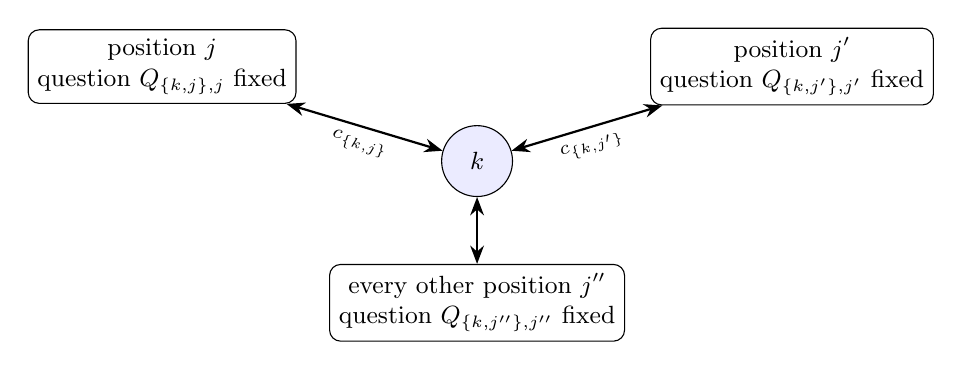
\begin{tikzpicture}[>=Stealth, every node/.style={font=\small}]
\node[draw,circle,minimum size=9mm,fill=blue!8] (k) at (0,0) {$k$};
\node[draw,rounded corners,align=center] (j) at (-4,1.2) {position $j$\\question $Q_{\{k,j\},j}$ fixed};
\node[draw,rounded corners,align=center] (l) at (4,1.2) {position $j' $\\question $Q_{\{k,j'\},j'}$ fixed};
\node[draw,rounded corners,align=center] (a) at (0,-1.8) {every other position $j''$\\question $Q_{\{k,j''\},j''}$ fixed};
\draw[<->,thick] (k)--node[below,sloped,font=\scriptsize] {$c_{\{k,j\}}$} (j);
\draw[<->,thick] (k)--node[below,sloped,font=\scriptsize] {$c_{\{k,j'\}}$} (l);
\draw[<->,thick] (k)--(a);
\end{tikzpicture}
\caption{The star operation centered at $k$. Each incident seed is
resampled within the fiber of its question at the opposite endpoint.
All nonincident seeds and all weights stay fixed. Thus every query
except the query at $k$ stays fixed. The schematic depicts the
conditional averaging operator $D_k$, not additional graph edges.}
\label{fig:star}
\end{figure}


For a component designated at \(j\), we charge invisible information
on \(\{j,k\}\) to the star centered at \(k\): that star retains
\(j\)'s question on this pair. For every \(j\ne k\), the range
of \(D_k\) is contained in that of
\(O_{\{k,j\},j}\).  Distance to the larger closed subspace is no
greater than distance to the smaller one.  Thus, for every \(v\in L^2\),
\[
 \|(\operatorname{Id}-O_{\{k,j\},j})v\|_2^2
       \leq\|(\operatorname{Id}-D_k)v\|_2^2.
\]
For fixed \(S\) and \(k\ne j(S)\), its seed decomposition shows that
\((\operatorname{Id}-O_{\{k,j(S)\},j(S)})f_S\) is the sum of exactly
the components with \(k\in N_{S,\omega}\).  Consequently
\begin{align}
 \sum_{S,\omega}|N_{S,\omega}|\|f_{S,\omega}\|_2^2
  &=\sum_{S\ne\varnothing}\sum_{k\ne j(S)}
    \|(\operatorname{Id}-O_{\{k,j(S)\},j(S)})f_S\|_2^2
       \notag\\
  &\leq\sum_{k=1}^d\sum_{S\ne\varnothing}
       \|(\operatorname{Id}-D_k)f_S\|_2^2
       \notag\\
  &=\sum_{k=1}^d\|(\operatorname{Id}-D_k)f\|_2^2
    \leq4d.\label{res:residual-degree}
\end{align}
The inequality applies the preceding projection bound and adds the
nonnegative terms with \(j(S)=k\). The next
equality uses the fact that \(D_k\) commutes with the weight projections,
so the images of distinct \(f_S\)'s remain orthogonal.  This argument
uses neither products of different \(D_k\)'s nor commutation of
opposite endpoint projections on one seed.

The three energy budgets are now available: weight interactions cost
at most \(4d\), all nonconstant seeds at most \(8d^2\), and incident
information hidden from the designated question at most \(4d\).
We next check exactly which of these components a restriction preserves.

\paragraph{What the restriction keeps.}
For fixed \(J\) and \(j\in J\), define the projection
\begin{equation}\label{res:restriction-operator}
 K_{J,j}=
 W_j^1\prod_{k\in J\setminus\{j\}}W_k^0
 \prod_{e\in\binom{J\setminus\{j\}}2}P_e^0
 \prod_{k\in J\setminus\{j\}}O_{\{j,k\},j}.
\end{equation}
All seed factors here act on distinct coordinates.  Before applying
\(W_j^1\), these operators average exactly the unfrozen data other than
the own questions \(u_j\) and the own weights \(s_j\).  They retain
the frozen data \(\mathbf a\) as variables.  The final centering
\(W_j^1\) subtracts the mean in \(s_j\), which is independent of
the retained seed information.  Thus
\[
 K_{J,j}f
  =H_j^{J,\mathbf a}(u_j,s_j)
    -\E_{s'_j}H_j^{J,\mathbf a}(u_j,s'_j)
\]
as functions on the original product space.  If
\[
 \mathcal V(J,\mathbf a)=
     \sum_{j\in J}\E_{u_j}\Var_{s_j}H_j^{J,\mathbf a}(u_j,s_j),
\]
then integration over the initially random frozen data gives
\begin{equation}\label{res:restriction-variance}
 \E_{\mathbf a}\mathcal V(J,\mathbf a)
     =\sum_{j\in J}\|K_{J,j}f\|_2^2.
\end{equation}
This identity uses only independent seed coordinates.  Conditioning on
the own questions restricts each incident hidden seed to its own fiber,
as in the definition of \(H_j\).

Consider \(f_{S,\omega}\) and its designated position \(j=j(S)\).
This component is preserved by the term \(K_{J,j}\) whenever
\begin{equation}\label{res:survival}
 S\cap J=\{j\},\qquad
 N_{S,\omega}\cap J=\varnothing,\qquad
 T_{S,\omega}\cap\binom{J\setminus\{j\}}2=\varnothing.
\end{equation}
To verify that its squared norm can be counted in
\eqref{res:restriction-variance}, first note that \(K_{J,j}\) commutes
with every \(\Pi_S\).  Thus its outputs from different weight supports
are orthogonal, and
\(\|K_{J,j}f\|_2^2=\sum_S\|K_{J,j}f_S\|_2^2\).
The weight factors in \(K_{J,j}\) keep \(f_S\) precisely when
\(S\cap J=\{j\}\).  For those \(S\) whose designated position is
this \(j\), the seed factors are diagonal in the chosen seed
decomposition: \(P_e^0\) on a nonincident hidden seed keeps just its
constant component, and \(O_{e,j}\) on an incident hidden seed keeps
its constant and own-question components.  The other seed coordinates
are untouched.  They therefore keep exactly the components satisfying
the last two conditions of \eqref{res:survival}, with no cancellation
among them.  We may discard all other nonnegative squared norms in
\eqref{res:restriction-variance} and count each component solely in its
designated term.  It follows that
\begin{equation}\label{res:surviving-energy}
 \E_{\mathbf a}\mathcal V(J,\mathbf a)
   \geq\sum_{S,\omega}
       \mathbf1_{\{\text{conditions \eqref{res:survival} hold}\}}
       \|f_{S,\omega}\|_2^2.
\end{equation}

\paragraph{Averaging the restriction.}
Choose \(J\) uniformly among all \(h\)-element subsets of \([d]\).
For a fixed component, the designated position belongs to \(J\) with
probability \(h/d\).  Conditional on this inclusion, a specified other
position belongs to \(J\) with probability
\[
 p_1=\frac{h-1}{d-1},
\]
and a specified pair avoiding the designated position lies in \(J\)
with probability
\[
 p_2=\frac{(h-1)(h-2)}{(d-1)(d-2)}.
\]
The first two conditions in \eqref{res:survival} fail only if one of
\(S\setminus\{j(S)\}\) or \(N_{S,\omega}\) is included.  The third
can fail only at a pair in \(T_{S,\omega}\) avoiding \(j(S)\).
A union bound therefore gives conditional survival probability at least
\begin{equation}\label{res:survival-probability}
 1-p_1\bigl(|S|-1+|N_{S,\omega}|\bigr)-p_2|T_{S,\omega}|.
\end{equation}
Charging all of \(T_{S,\omega}\) only decreases this lower bound.
The bound remains valid when the displayed expression is negative.

By \eqref{res:weight-degree}, \eqref{res:residual-degree}, and the
orthogonal refinement of each \(f_S\),
\[
 \sum_{S,\omega}\bigl(|S|-1+|N_{S,\omega}|\bigr)
             \|f_{S,\omega}\|_2^2\leq8d.
\]
Combining \eqref{res:component-energy}, \eqref{res:seed-degree},
\eqref{res:surviving-energy}, and \eqref{res:survival-probability}
now yields
\begin{align}
 \E_{J,\mathbf a}\mathcal V(J,\mathbf a)
   &\geq\frac hd\bigl(\|f\|_2^2-8dp_1-8d^2p_2\bigr)\notag\\
   &\geq\frac hd\bigl(\nu d-16h-32h^2\bigr)
    \geq\frac{\nu h}{2}.\label{res:averaged-variance}
\end{align}
For the second inequality, \(d\geq4\) gives
\(p_1\leq2h/d\) and \(p_2\leq4h^2/d^2\); the last inequality
is \eqref{res:scale}.

The nonnegative measurable quantity \(\mathcal V(J,\mathbf a)\) is
bounded, since \(f\) is bounded.  Its mean in
\eqref{res:averaged-variance} implies that a set of choices
\((J,\mathbf a)\) of positive probability has
\(\mathcal V(J,\mathbf a)\geq\nu h/4\).  Choose one such restriction.
The conditional averages were defined by explicit integration with its
frozen coordinates plugged in.  All hidden seeds and batch weights are
then drawn with their original product law, establishing
\eqref{res:variance} with the asserted interpretation.
\end{proof}

\section{Lists from own-question conditional means}
\label{ana:private-section}

The restriction lemma retains variance in conditional means that see
only one position's own questions and weights. We use this variance
to produce short lists of local labels. Set
\begin{equation}
 \beta=\frac\nu8,\qquad \ell=\frac2\beta,\qquad h=2\ell.
 \label{src:list-parameters}
\end{equation}
Since \(\nu=1/(2^7m^3)\), both \(\ell\) and \(h\) are
positive integers depending only on \(m\). Assume from now on that
the number \(d\) of graph positions also satisfies
\begin{equation}
 h<d,\qquad 16h+32h^2\leq\frac{\nu d}{2}.
 \label{src:restriction-budget}
\end{equation}
The joint parameter choice in \Cref{sec:conclusion} will ensure
these conditions. Applying \Cref{res:private-variance} to the
function in \Cref{ana:function} supplies a fixed set
\(J\subset[d]\) of size \(h\) and fixed data \(\boldsymbol a\)
consisting of the weights outside \(J\) and every seed outside
\(\mathcal E_J=\binom J2\). Write
\(f^*(\boldsymbol c_J,\boldsymbol s_J)\) for \(f\) with these
values plugged in. In the rest of this section the probability law
is the product of independent uniform hidden seeds
\((c_e)_{e\in\mathcal E_J}\) and independent uniform weight blocks
\((s_j)_{j\in J}\) on \([-1,1]^r\). The choice of the fixed data
does not condition these remaining draws on any event of success.

For \(j\in J\), write
\(u_j=(q_{jk})_{k\in J\setminus\{j\}}\), in increasing order of
\(k\), for the tuple of questions received by \(j\) from its
incident hidden seeds. Together with \(\boldsymbol a\), it
specifies the whole query \(i_j\); denote the completed query by
\(i_j(u_j)\). The conditional averages supplied by the restriction
lemma satisfy
\begin{equation}
 \sum_{j\in J}\E_{u_j}\Var_{s_j}H_j(u_j,s_j)
       \geq\nu h/4.
 \label{ana:restricted-variance}
\end{equation}
Here \(H_j(u,s)\) is the mean of \(f^*\) given the own questions
\(u_j=u\) and the own weight block \(s_j=s\).
Our aim is to turn this variance into own-input lists of size at most
\(\ell\) whose maximum compatible hit count has expectation at
least two.

To differentiate these means, we use the explicit integral from
\Cref{sec:restriction}. For a tuple \(u\) in
\(\supp u_j\), let \(\kappa_j(u)\) be the conditional distribution of
all hidden seeds given \(u_j=u\). On an incident pair
\(\{j,k\}\), this is uniform on the occurrence indices producing
the specified question at \(j\); on a nonincident hidden pair it
is uniform on \([M]\). All these conditional seed coordinates are
independent. This follows from independence of the original seeds
and from the fact that each condition fixes a function of just one
seed. Thus
\begin{equation}
 H_j(u,s)=
  \E_{\boldsymbol c_J\sim\kappa_j(u),\,(s_k)_{k\in J\setminus\{j\}}}
            f^*(\boldsymbol c_J,\boldsymbol s_J)
               \big|_{s_j=s},
 \label{ana:own-mean}
\end{equation}
where the other weight blocks have their original independent
uniform laws. The seed law in this formula does not depend on
\(s\). We use zero as a fallback for \(H_j\) on unsupported own
question tuples. The fixed data throughout are \(\Phi,F,J\), and
\(\boldsymbol a\).

\subsection{One gradient rule on every tuple}

The increments at positions outside \(J\) are fixed: their queries
use no seed in \(\mathcal E_J\). Set
\[
 c_0=\sum_{k\notin J}z(i_k,s_k).
\]
For a fixed tuple of batch queries \(\boldsymbol i=(i_j)_{j\in J}\),
consider the function on the whole real weight space
\[
 \psi_{\boldsymbol i}(\boldsymbol s_J)
       =F\left(c_0+\sum_{j\in J}z(i_j,s_j)\right).
\]
For \(I\in\mathcal I\), let
\(v_I(\boldsymbol i)\in\R^{J\times[r]}\) have entry one at
\((j,\operatorname{slot}_{i_j}(\lambda))\) if
\((i_j,\lambda)\in I\), and zero elsewhere. It has at most one
nonzero entry in each block \(j\).
We will represent the gradient using these incidence vectors. At
exceptional weights where a derivative need not exist, the same
representation will hold for a prescribed value of the gradient rule.

\begin{lemma}[A gradient rule in the compatibility hull]
\label{ana:gradient}
There is a deterministic measurable rule
\(g=(g_j)_{j\in J}\in\R^{J\times[r]}\), defined at every batch
query and real-weight tuple, that equals
\(\nabla\psi_{\boldsymbol i}\) outside a finite union of proper
affine hyperplanes for each fixed query tuple and fixed frozen
data. At every tuple,
\begin{equation}
 g\in\conv\{\pm v_I(\boldsymbol i):I\in\mathcal I\}.
 \label{ana:hull}
\end{equation}
Consequently,
\begin{equation}
 \|g_j\|_1\leq1,
 \qquad
 g_{j,t'}=0\quad\hbox{if }t'\notin
                   \operatorname{slot}_{i_j}(\Lambda_{i_j}).
 \label{ana:block-bound}
\end{equation}
The rule uses the fixed formula for \(F\), the frozen increments,
and the supplied batch queries and weights. It does not inspect
which hidden seed occurrences produced those queries.
\end{lemma}

\begin{proof}
Let \(\ind_I\in\R^{\mathcal P}\) be the indicator vector of
\(I\). For \(\zeta\in A_*\cup(-A_*)\),
\(I\in\mathcal I\), and \(\varepsilon\in\{-1,1\}\), form the
finite collection of affine expressions
\begin{equation}
 L_{\zeta,I,\varepsilon}(\boldsymbol s_J)
    =\varepsilon\langle\ind_I,c_0-\zeta\rangle
       +\varepsilon\langle v_I(\boldsymbol i),\boldsymbol s_J\rangle.
 \label{ana:affine-candidates}
\end{equation}
For either \(\mathcal C=A_*\) or \(\mathcal C=-A_*\),
\[
 \dist_*\left(c_0+\sum_{j\in J}z(i_j,s_j),\mathcal C\right)
   =\min_{\zeta\in\mathcal C}
       \max_{I\in\mathcal I,\,\varepsilon\in\{-1,1\}}
                    L_{\zeta,I,\varepsilon}(\boldsymbol s_J).
\]
In particular, \(\psi_{\boldsymbol i}\) is continuous and piecewise
affine, with finitely many pieces.

Compare all pairs of candidates in \eqref{ana:affine-candidates}.
If two candidates with different slope vectors in the unfrozen
weights tie in value, set \(g=0\). Otherwise take the true gradient
of the finite formula for \(\psi_{\boldsymbol i}\). This latter
choice is well-defined. Two candidates with the same slope either
never tie or are identical affine functions. All other comparisons
are strict at such a point and persist in a neighborhood; each
minimum and maximum there selects one affine function up to
identical copies. The resulting formula is affine in that
neighborhood. Fixing a deterministic order on candidates resolves
any choice between identical copies without changing its gradient.

Each discarded equality has a nonzero normal in the unfrozen
coordinates, hence defines a proper affine hyperplane. No choice of
frozen weights changes that fact, since frozen weights change the
offsets but not the slopes. Identical slopes caused by repeated
endpoint questions or other coincidences are allowed. Finite
comparisons prove measurability, and the rule is defined even at
query tuples that cannot arise from the hidden seed law. Its formula
uses the queries themselves and no additional seed information.

At a point not discarded, choose an active affine expression in
each distance formula. Write their slopes as
\(\varepsilon_-v_{I_-}(\boldsymbol i)\) for the distance to
\(-A_*\) and \(\varepsilon_+v_{I_+}(\boldsymbol i)\) for the
distance to \(A_*\). Since \(F\) is half the difference of
these distances,
\[
 g=\frac12\bigl(\varepsilon_-v_{I_-}(\boldsymbol i)
                  -\varepsilon_+v_{I_+}(\boldsymbol i)\bigr).
\]
Both vectors in this average are signed compatible-incidence
vectors, proving \eqref{ana:hull}. At discarded points the chosen
value zero also belongs to the symmetric hull. Every signed
incidence vector has block \(\ell^1\) norm at most one and zero
entries in the unused slots, so convexity proves
\eqref{ana:block-bound} at every tuple.
\end{proof}

\subsection{Own-question conditional gradients}

For supported \(u\) and any \(s\in\R^r\), define
\begin{equation}
 \bar g_j(u,s)=
   \E_{\boldsymbol c_J\sim\kappa_j(u),\,(s_k)_{k\in J\setminus\{j\}}}
               g_j(\boldsymbol c_J,\boldsymbol s_J)\big|_{s_j=s}.
 \label{ana:conditional-gradient}
\end{equation}
Here the notation for \(g_j\) means that the seed tuple is used
only to form the queries supplied to the rule in
\Cref{ana:gradient}. Set \(\bar g_j(u,s)=0\) for unsupported
own tuples. For supported \(u\), its query \(i_j(u)\) is fixed
throughout the integral. Convexity and \eqref{ana:block-bound} give,
at every own input,
\begin{equation}
 \|\bar g_j(u,s)\|_1\leq1,
 \qquad
 \bar g_{j,t'}(u,s)=0\quad\hbox{on unused slots of }i_j(u).
 \label{ana:mean-block-bound}
\end{equation}

\begin{lemma}[Conditional cube variance]
\label{ana:cube}
For each \(j\in J\) and supported own tuple \(u\), the function
\(H_j(u,\cdot)\) is \(1\)-Lipschitz with respect to
\(\|\cdot\|_\infty\). For almost every own
\(s\in[-1,1]^r\),
\begin{equation}
 \partial_{s^{(t')}}H_j(u,s)=\bar g_{j,t'}(u,s),
 \qquad t'\in[r].
 \label{ana:conditional-derivative}
\end{equation}
Its variance satisfies the dimension-independent bound
\begin{equation}
 \Var_s H_j(u,s)
       \leq2\E_s\|\bar g_j(u,s)\|_2^2.
 \label{ana:cube-variance}
\end{equation}
Consequently, under the fixed restricted law,
\begin{equation}
 \sum_{j\in J}\E\|\bar g_j(u_j,s_j)\|_2^2
      \geq\nu h/8=\beta h.
 \label{ana:energy}
\end{equation}
\end{lemma}

\begin{proof}
Replacing the own block \(s\) by \(s'\), with a seed configuration
and other weights fixed, changes the integrand in
\eqref{ana:own-mean} by at most \(\|s-s'\|_\infty\). The same
bound holds after averaging. In particular, every scalar-coordinate
difference quotient of the integrand is bounded in absolute value
by one.

For each fixed hidden seed tuple, the full gradient identification
in \Cref{ana:gradient} holds outside a null set in all batch weights.
Fubini implies that for almost every own \(s\) it holds for almost
all other weight blocks. The conditional seed law \(\kappa_j(u)\) has
finite support and does not depend on \(s\), so the exceptional sets
may be united over its support and over the finitely many weight
coordinates. At the remaining own values, the coordinate difference
quotients converge almost surely to \(g_{j,t'}\). Dominated
convergence gives \eqref{ana:conditional-derivative}; the boundary
of the cube has measure zero.

Every coordinate-line restriction of \(H_j(u,\cdot)\) is
Lipschitz and hence absolutely continuous. By Fubini applied to
\eqref{ana:conditional-derivative}, for almost every fixing of the
other own coordinates its derivative agrees almost everywhere with
the corresponding entry of \(\bar g_j\). The fundamental theorem
of calculus therefore expresses differences between any two values
on such a line as the integral of that entry.

Let \(w_0\) be the restriction of \(H_j(u,\cdot)\) to one of these
lines. For \(x,y\in[-1,1]\), Cauchy--Schwarz gives
\[
 |w_0(x)-w_0(y)|^2
    \leq |x-y|\int_{\min(x,y)}^{\max(x,y)}|w_0'(z)|^2\,dz
    \leq2\int_{-1}^1|w_0'(z)|^2\,dz.
\]
For independent uniform \(X,Y\in[-1,1]\), this implies
\[
 \Var(w_0(X))=\tfrac12\E|w_0(X)-w_0(Y)|^2
      \leq\int_{-1}^1|w_0'(z)|^2\,dz
      =2\E|w_0'(X)|^2.
\]
The product decomposition of Efron and
Stein~\cite[Section~2]{EfronStein1981} bounds variance by the sum
of the averaged one-coordinate conditional variances. To see this
consequence directly,
decompose the identity at each scalar coordinate into its averaging
projection and its orthogonal complement. The resulting orthogonal
components are indexed by subsets of coordinates. Total variance
counts every nonconstant squared component once, while the sum of
one-coordinate conditional variances counts it once for each member
of its nonempty index subset. Applying the line estimate,
integrating over the other coordinates, and summing proves
\eqref{ana:cube-variance}. Averaging that bound over the own tuples
and summing over \(j\), then using
\eqref{ana:restricted-variance}, proves \eqref{ana:energy}.
\end{proof}

A particular own weight value can make an entire slice of the other
weights exceptional. The derivative identity is only an
almost-everywhere assertion, and \eqref{ana:energy} is integrated
over the restricted law. In contrast,
\eqref{ana:hull}, \eqref{ana:block-bound}, and
\eqref{ana:mean-block-bound} hold at every input of their respective
rules, including exceptional weights.

\subsection{Thresholding the conditional gradients}

The conditional means now retain total squared gradient energy at
least \(\beta h\), and each block has \(\ell^1\) norm at most one.
Keeping coordinates above a fixed threshold therefore gives short
lists without an alphabet-size factor. The remaining task is to
transfer their mass back to the single full gradient, whose compatible
incidence representation can certify simultaneous hits.

For supported \(u\), define the slot-ordered list
\begin{equation}
 \mathcal L_j(u,s)=
  \left\{\lambda\in\Lambda_{i_j(u)}:
    \left|\bar g_{j,\operatorname{slot}_{i_j(u)}(\lambda)}(u,s)\right|
       \geq\frac\beta2\right\}.
 \label{ana:list-definition}
\end{equation}
For an unsupported own question tuple, let the list be empty.
At an actual draw write \(L_j=\mathcal L_j(u_j,s_j)\), and define
\begin{equation}
 Z=\max_{I\in\mathcal I}
       \#\{j\in J:\exists\lambda\in L_j\text{ with }(i_j,\lambda)\in I\}.
 \label{ana:hit-count}
\end{equation}

\begin{proposition}[Local lists and compatible hits]
\label{ana:lists}
The functions \(\mathcal L_j\) are deterministic total measurable maps
returning at most \(\ell\) valid labels. Once
\(\Phi,F,J,\boldsymbol a\) and the conditional kernels above are
fixed, each list uses only its own questions \(u_j\) and weights
\(s_j\). In particular it has no additional access to the actual
hidden seed occurrences or to any other actual batch input.
Under the fixed restricted product law,
\begin{equation}
 \E Z\geq\frac{\beta h}{2}=2.
 \label{ana:list-hits}
\end{equation}
\end{proposition}

\begin{proof}
The mean block bound gives
\[
 \frac\beta2|\mathcal L_j(u,s)|\leq\|\bar g_j(u,s)\|_1\leq1,
 \qquad |\mathcal L_j(u,s)|\leq2/\beta=\ell.
\]
It also gives zero dummy entries, so thresholding returns only valid
labels. Finite threshold comparisons of measurable functions, with
an empty-list fallback, prove totality and measurability.

We first transfer the retained mass of the own conditional means
to the full gradient rule \(g\), and then apply its pointwise hull bound.
For an actual own input, let \(T_j\subset[r]\) be the set of slots
of \(L_j\), and write \(\mathcal G_j\) for the information
\((u_j,s_j)\). The conditional mean in
\eqref{ana:conditional-gradient} is a version of
\(\E[g_j\mid\mathcal G_j]\), defined by the displayed kernel even
at own values of probability zero. For slots outside \(T_j\),
\eqref{ana:mean-block-bound} and the threshold give
\[
 \sum_{t'\notin T_j}|\bar g_{j,t'}|^2
       \leq\frac\beta2\sum_{t'\notin T_j}|\bar g_{j,t'}|
       \leq\frac\beta2.
\]
For the list slots, each mean entry has magnitude at most one, and
conditional Jensen gives
\[
 \sum_{t'\in T_j}|\bar g_{j,t'}|^2
   \leq\sum_{t'\in T_j}|\bar g_{j,t'}|
   \leq\E\left[\sum_{t'\in T_j}|g_{j,t'}|
                         \,\middle|\,\mathcal G_j\right].
\]
The last inequality uses the fact that \(T_j\) is determined by
\(\mathcal G_j\). Taking expectations, summing, and applying
\eqref{ana:energy} therefore yields
\begin{equation}
 \E\sum_{j\in J}\sum_{\lambda\in L_j}
        |g_{j,\operatorname{slot}_{i_j}(\lambda)}|
       \geq\beta h-\frac\beta2h=\frac{\beta h}{2}.
 \label{ana:retained-mass}
\end{equation}

For arbitrary fixed queries and arbitrary lists of valid labels,
the sum of absolute values over their slot sets is a convex
function of the full vector in \(\R^{J\times[r]}\). On a signed
generator \(\pm v_I(\boldsymbol i)\) it equals the number of
positions hit by that selection \(I\), since each block contains
at most one selected slot. Its value on every point of the hull
in \eqref{ana:hull} is consequently at most the maximum such hit
count. At every realized tuple, apply this deterministic statement
to the realized lists and the full vector \(g\):
\begin{equation}
 \sum_{j\in J}\sum_{\lambda\in L_j}
        |g_{j,\operatorname{slot}_{i_j}(\lambda)}|\leq Z.
 \label{ana:pointwise-hits}
\end{equation}
No independence between the lists and the gradient, or between
positions, is required. Combining \eqref{ana:retained-mass} and
\eqref{ana:pointwise-hits} proves \eqref{ana:list-hits}, with
\(\beta h/2=2\) from \eqref{src:list-parameters}.

Finally, \eqref{ana:own-mean} and
\eqref{ana:conditional-gradient} integrate over hidden seeds
against the fixed law \(\kappa_j(u)\), and over other weights against
their fixed cube laws. Their actual realized values are not inputs
to the resulting mean function. Thus \eqref{ana:list-definition}
has exactly the stated own-input dependence. No efficiency of this
rule is needed for the soundness argument.
\end{proof}

The kernels and list maps in this section remain fixed throughout
the subsequent argument. Conditioning later on other hidden seeds
or on all weights changes the distribution of the inputs to these
maps; it does not recompute their conditional averages. Locality,
validity, and list-size bounds continue to hold for every fixed
weight choice. The lower bound \eqref{ana:list-hits} concerns the
original restricted product law.

\section{Pair decoding and soundness}
\label{dec:section}

Set
\begin{equation}
 \sigma=\frac1{h^2\ell^2},
 \label{src:decoding-soundness}
\end{equation}
and assume throughout this section that \(\val(\Phi)\leq\sigma\).
The source promise bounds every labeling of \(U\cup V\), so the
decoders below may use arbitrary fixed instance-dependent data.
Their essential restriction is that the label returned at a variable
does not also depend on the sampled constraint occurrence.

Fix a set \(J\subseteq[d]\) of size \(h\) and frozen data
\(\mathbf a\) as in \Cref{res:private-variance}. The remaining
seeds \(c_e\), \(e\in\binom J2\), are independent uniform
elements of \([M]\); the weight blocks \(s_j\), \(j\in J\),
are independent uniforms on \([-1,1]^r\), independent of the
seeds. Let \(u_j\) be position \(j\)'s tuple of questions from
its incident hidden seeds. Together with \(\mathbf a\), this
tuple determines its query \(i_j\).

Consider any fixed total measurable maps
\begin{equation}
 L_j=\mathcal L_j(u_j,s_j)\subseteq\Lambda_{i_j},
 \qquad |L_j|\leq\ell.
 \label{dec:local_lists}
\end{equation}
Each map receives only the indicated own questions and weights;
on an unsupported own-question tuple it returns the empty list.
Order each list by its slots. The lists in \Cref{ana:lists} have
exactly these properties.

For distinct \(j,k\in J\), let \(E_{jk}\) be the event that
some \(I\in\mathcal I\) hits both lists: it contains
\((i_j,\lambda_j)\) and \((i_k,\lambda_k)\) for labels
\(\lambda_j\in L_j\), \(\lambda_k\in L_k\). Define
\begin{equation}
 Z=\max_{I\in\mathcal I}
       \#\{j\in J:\text{ some }\lambda\in L_j
                              \text{ has }(i_j,\lambda)\in I\}.
 \label{dec:hits}
\end{equation}

\begin{lemma}[Decoding a pair]
\label{dec:pair}
For every fixed \(J,\mathbf a\) and fixed list maps satisfying
\Cref{dec:local_lists},
\begin{equation}
 \Pr(E_{jk})\leq\ell^2\sigma
 \quad(j,k\in J,\ j<k),
 \qquad
 \E Z\leq1+\binom h2\ell^2\sigma
       =\frac32-\frac1{2h}<\frac32.
 \label{dec:pair_bound}
\end{equation}
\end{lemma}
\begin{proof}
Fix \(j<k\) and write \(e=\{j,k\}\). Fix all batch weights
and all hidden seeds except \(c_e\). By independence, the
remaining occurrence \(c_e\) is still uniform on \([M]\).
Position \(j\)'s only varying question is \(x_{c_e}\in U\),
and position \(k\)'s only varying question is \(y_{c_e}\in V\).
Every other argument of each list map is now a constant, while the
maps themselves remain fixed. For the maps constructed in
\Cref{ana:lists}, their conditional averages are not recomputed:
the actual values just fixed are not supplied as new arguments to
those averages.

For \(x\in U\), form the tuple \(u_j^{x}\) by putting \(x\)
in the distinguished \(e\)-coordinate of \(u_j\) and retaining
all its other, now fixed, coordinates. Define \(u_k^{y}\) for
\(y\in V\) in the same way. Choose default symbols
\(a_U\in\Sigma_U\) and \(a_V\in\Sigma_V\). For each pair
of ranks \(\rho,\tau\in[\ell]\), define a labeling
\(A_{\rho,\tau}\) of the entire source instance as follows.
At a variable \(x\in U\), evaluate
\(\mathcal L_j(u_j^{x},s_j)\). If rank \(\rho\) is present,
give \(x\) its value in that label; otherwise give it \(a_U\).
At a variable \(y\in V\), use its value in the label at rank
\(\tau\) of \(\mathcal L_k(u_k^{y},s_k)\), or \(a_V\) if
the rank is absent.

This gives one symbol at every source variable. If a substituted
tuple has probability zero, its empty list invokes the same
fallback. If the variable already occurs in another coordinate of
the query, its value in a present label is still unique: a local
label is an assignment on the set of distinct variables in the
scope. Thus repeated variables, empty valid-label sets, and missing
ranks cause no ambiguity. The assigned symbol on \(U\) depends
only on \(x\), and the assigned symbol on \(V\) only on \(y\),
besides fixed data. It does not use the occurrence index or its
projection map. The source promise consequently gives
\begin{equation}
 \Pr_{c\text{ uniform in }[M]}
 \bigl[\pi_c(A_{\rho,\tau}(x_c))
                    =A_{\rho,\tau}(y_c)\bigr]\leq\sigma.
 \label{dec:rank_soundness}
\end{equation}

For every actual remaining occurrence \(c_e\), the reconstructed
tuples \(u_j^{x_{c_e}},u_k^{y_{c_e}}\) are supported under the
original hidden-seed law: the full seed tuple comprising the fixed
other seeds and this occurrence has positive probability in that
product law. They are exactly the own tuples at which the actual
lists are evaluated.

Suppose \(E_{jk}\) occurs and choose the ranks \(\rho,\tau\)
of labels witnessing it. The endpoint \(x_{c_e}\) belongs to
\(P(i_j)\), and \(y_{c_e}\) to \(P(i_k)\). Compatibility
requires the induced labeling to satisfy every source constraint
with both endpoints in the union of the selected scopes. In
particular it satisfies the sampled occurrence \(c_e\). Its
endpoint labels are exactly those used by
\(A_{\rho,\tau}\), so
\[
 \pi_{c_e}(A_{\rho,\tau}(x_{c_e}))
                 =A_{\rho,\tau}(y_{c_e}).
\]
This uses the sampled occurrence even when other occurrences have
the same endpoints. Union bounding \Cref{dec:rank_soundness} over
the \(\ell^2\) rank pairs proves the pair estimate for the fixed
weights and other seeds. It is uniform in those fixed values, so
averaging proves \(\Pr(E_{jk})\leq\ell^2\sigma\). No
conditioning on compatible labels or successful ranks is used.

For every integer \(z\geq0\),
\(z\leq1+\binom z2\), since the difference is
\((z-1)(z-2)/2\geq0\). Choose a selection attaining the maximum
in \Cref{dec:hits}. Each of the pairs among its \(Z\) hit
positions witnesses the corresponding event \(E_{jk}\).
Consequently, pointwise,
\begin{equation}
 Z\leq1+\binom Z2
   \leq1+\sum_{\{j,k\}\in\binom J2}\ind_{E_{jk}}.
 \label{dec:pair_count}
\end{equation}
Taking expectations, using the pair estimate, and substituting
\(\sigma=1/(h^2\ell^2)\) gives \Cref{dec:pair_bound}.
\end{proof}

\begin{corollary}[Soundness]
\label{dec:soundness}
For the graph constructed in \Cref{graph:section}, assume
\eqref{src:restriction-budget}.
If \(\val(\Phi)\leq\sigma\), every independent set has size
strictly less than \(n/m\).
Consequently \(\tau(G)>(1-1/m)n\).
\end{corollary}
\begin{proof}
Suppose an independent set \(\mathcal A\) has size at least
\(n/m=2b_0n\). By the low-norm clique observation at the start of
\Cref{ana:section}, at most one vertex of \(\mathcal A\) has
\(\norm{S_v}\leq t\). Since \(n\geq p>1/b_0\), the number
of its high-norm vertices is at least
\[
 2b_0n-1>b_0n.
\]

\Cref{ana:function} therefore supplies the single fixed odd
Lipschitz function \(F\) and its variance lower bound. Applying
\Cref{res:private-variance} and then the list construction of
\Cref{ana:lists,ana:list-hits} gives fixed \(J,\mathbf a\)
and local lists with
\[
 \E Z\geq\frac{\beta h}{2}=2.
\]
This contradicts \Cref{dec:pair}, which gives \(\E Z<3/2\)
under the same remaining product law.

The lower bound just used averages over the hidden seeds and
continuous batch weights for those fixed \(J,\mathbf a\).
The upper bound fixes further weights and seeds only to decode a
single occurrence and is then averaged back. It does not require
an energy lower bound, or a derivative identity, at every such
further fixing.

We have ruled out every independent set of size at least \(n/m\).
The complement of any vertex cover is independent, so every cover
has size strictly greater than \(n-n/m\), as claimed.
\end{proof}

\section{The approximation threshold}
\label{sec:conclusion}

The construction and soundness analysis were stated with explicit
requirements on their constants. We now choose those constants jointly,
before requesting the source alphabets.

For the given integer \(m\geq4\), the definitions in
\Cref{src:construction-parameters,src:variance-parameters,src:list-parameters,src:decoding-soundness}
are completed by choosing \(d=2^{38}m^{10}\). Thus
\begin{equation}
\begin{aligned}
 a&=\frac1{4m},& b_0&=\frac1{2m},
 &\nu&=\frac1{2^7m^3},\\
 \beta&=\frac1{2^{10}m^3},&\ell&=2^{11}m^3,
 &h&=2^{12}m^3,\\
 d&=2^{38}m^{10},&\sigma&=\frac1{2^{46}m^{12}},
 &p&=2d+1,\\
 t&=2^{17}m^4.
\end{aligned}
\label{src:parameters}
\end{equation}
The construction conditions \eqref{src:dimension-bounds} hold because
\(d\) is even and \(\sqrt d=2^{19}m^5>4m\). For the restriction
conditions \eqref{src:restriction-budget}, we have \(h<d\) and
\[
 16h+32h^2=2^{16}m^3+2^{29}m^6
 \leq2^{30}m^7=\frac{\nu d}{2}.
\]
The displayed inequality holds already for \(m\geq1\).
The remaining list and decoding identities are
\[
 \frac{\beta h}{2}=2,\qquad
 \binom h2\ell^2\sigma=\frac{h-1}{2h}<\frac12.
\]
All choices depend only on \(m\); no label alphabet has entered them.
Their magnitude affects the constants and degree of the polynomial
running time, but every fixed \(m\) gives a fixed reduction.

\begin{proof}[Proof of \Cref{thm:gap,thm:hardness}]
Fix \(m\geq4\) and the constants in \Cref{src:parameters}.
Apply \Cref{src:hardness} at this \(\sigma\) to obtain fixed
source alphabets and a polynomial-time reduction from \(\mathrm{3SAT}\).
Now define \(q,r\) from those alphabets and construct the graph.
\Cref{graph:polynomial} makes its vertex and edge lists explicit in
deterministic polynomial time. All the hypotheses of
\Cref{graph:completeness,dec:soundness} have been verified above, so
these results give the two cover bounds in \Cref{thm:gap}.

For a fixed real \(\alpha\in[1,2)\), choose a fixed integer
\(m\geq4\) such that
\begin{equation}
 \alpha<R_m:=\frac{1-1/m}{1/2+1/m}
       =2-\frac6{m+2}.
\label{eq:gap-ratio}
\end{equation}
Suppose an algorithm always returns a vertex cover of size at most
\(\alpha\tau(G)\). On a completeness instance its output has
size strictly less than
\[
 \alpha\left(\frac12+\frac1m\right)n
 <\left(1-\frac1m\right)n,
\]
whereas on a soundness instance every cover has size strictly greater
than \((1-1/m)n\). Comparing the output cardinality with this
rational threshold distinguishes the two source cases. The comparison
uses only integer arithmetic: multiply the cardinality by \(m\)
and compare with \((m-1)n\). The real number \(\alpha\) is used
only to choose the fixed integer \(m\); it is not an input to the
reduction. This proves \Cref{thm:hardness}.
\end{proof}

For completeness, the matching upper bound on the approximation
factor is elementary. Find a maximal matching and return the set of
all its endpoints. Maximality makes this set a vertex cover: an edge
with neither endpoint selected could be added to the matching.
Every vertex cover contains an endpoint of each matching edge, and
these edges are disjoint. The returned cover therefore has size at
most twice optimum. Together with \Cref{thm:hardness}, this gives the
constant approximation threshold \(2\), unless
\(\mathrm P=\mathrm{NP}\).


\bibliographystyle{plain}
\bibliography{references}
\end{document}
